\documentclass{article}
\usepackage[utf8]{inputenc}

\title{\HUGE \textless Tu vstavi zelo dober naslov \textgreater}
\author{Rok Mlinar Vahtar}
\date{August 2023}
\usepackage[slovene]{babel}
\usepackage[none]{hyphenat}
\usepackage{subcaption}
\usepackage{mwe}
\usepackage{graphicx}
\usepackage[margin=1in]{geometry}
\usepackage{svg}
\usepackage{amsmath}
\usepackage{float}

\begin{document}

\maketitle

\section{Uvod}
\textless \hspace{1pt} tu vstavi fenomenalno napisan uvod \textgreater

\tableofcontents


\section{Standardni TFIM model}
Hamiltonian za standardni Isingov model z tranzverzalnim poljem se glasi
\begin{equation}
    \hat{H} = \sum_{< i,j >} -J \hat{\sigma_i^z} \hat{\sigma_j^z} - h\sum_i \hat{\sigma_i^x}
\end{equation}
in ga za dimenzije $N < 10$ lahko rešimo z eksaktno diagonalizacijo v doglednem času. 

 \subsection{Ekzaktna diagonalizacija TFIM modela}

 \subsubsection{Bazna stanja in Hamiltonian}
Da izvedemo eksaktno diagonalizacijo moramo najprej sestaviti matriko, ki predstavlja hamiltonian. Najprej moramo določiti bazo, ki jo bomo uporabljali, saj hočemo, da za vektor $\Vec{x}$, ki bo predstavljal stanje velja naslednje: $\Vec{x}^T \hat{H} \Vec{x} = E$, kjer je E energija tega stanja. Bazni vektorji morajo skupaj predstavljati vsa možna stanja z-projekcije vseh N spinov. Če si za bazo izberemo stanja, tako da je n-to stanje enako kot binarno zapisan n (Peto stanje je 0...000101), kjer 0 in 1 predstavljata spin dol in gor, lahko hamiltonian zapišmo kot tentzorski produkt Paulijevih matrik in identitet. To pomeni, da za vsak člen v zgornji vsoti, tenzorsko pomnožimo Paulijevi matriki na mestih i in j, ter identitete povsod drugod, v vrstnem redu, kot si sledijo spini v verigi. V primeru ko je $N = 3$ izgleda to tako:

\begin{center}
\begin{tabular}{c|c|c}
     Število stanja& Binarni zapis & Orientacija spinov\\
     \hline
     7& 111 & $\uparrow$ $\uparrow$ $\uparrow$\\
     6& 110 & $\uparrow$ $\uparrow$ $\downarrow$\\
     5& 101 & $\uparrow$ $\downarrow$ $\uparrow$\\
     4& 100 & $\uparrow$ $\downarrow$ $\downarrow$\\
     3& 011 & $\downarrow$ $\uparrow$ $\uparrow$\\
     2& 010 & $\downarrow$ $\uparrow$ $\downarrow$\\
     1& 001 & $\downarrow$ $\downarrow$ $\uparrow$\\
     0& 000 & $\downarrow$ $\downarrow$ $\downarrow$
\end{tabular}
\end{center}

\begin{equation}
    H = -J (\sigma^z \otimes \sigma^z \otimes I + I \otimes \sigma^z \otimes \sigma^z) - h (\sigma^x \otimes I \otimes I + I\otimes \sigma^x \otimes I + I \otimes I \otimes \sigma^x)
\end{equation}
kjer so:
\begin{equation}
    \sigma^z = \begin{bmatrix}1 & 0\\0 & -1\end{bmatrix} \hspace{1cm} \sigma^x = \begin{bmatrix}0 & 1\\1 & 0\end{bmatrix} \hspace{1cm} \begin{bmatrix}a1 & a2\\a3 & a4\end{bmatrix} \otimes \begin{bmatrix}b1 & b2\\b3 & b4\end{bmatrix} = \begin{bmatrix}
    a1 \begin{bmatrix}b1 & b2\\b3 & b4\end{bmatrix}  & a2 \begin{bmatrix}b1 & b2\\b3 & b4\end{bmatrix}\\
    a3 \begin{bmatrix}b1 & b2\\b3 & b4\end{bmatrix} & a4 \begin{bmatrix}b1 & b2\\b3 & b4\end{bmatrix}
    \end{bmatrix}
\end{equation}



\noindent Ko je matrika sestavljena jo le še diagonaliziramo z poljubnim algoritmom. Sam uporabljam python metodo scipy.linalg.eigsh, ki izkoristi hermitskost in redkost naše matrike, v zameno za to, da lahko izračuna le nekatere izmed lastnih vektorjev. Ker nas v resnici zanima le osnovno stanje, nam to ne dela težav, saj vedno lahko najdemo lastni vektor z najnižjo energijo.\\\\

 
\subsection{Magnetizacija}

\noindent Sedaj, ko imamo diagonaliziran hamiltonian, se lahko lotimo analize. Dobra mera za stanje sistema, ki nas bo tu zanimala, je magnetizacija, ki jo definiramo kot:
\begin{equation}
    M = \frac{1}{N}\sum_{i=0}^N \sigma_i^z
\end{equation}\\
Vse naslednje metode, predstavljene v tem poglavju se nahajajo v datoteki TFIM\_QuSpin.py .
Če fiksiramo J = 1 in variiramo h, ter vsakič izračunamo magnetizacijo, dobimo naslednji graf, ki kaže fazni prehod pri $h \approx J$. To opravlja funkcija main().
\begin{figure}[H]
    \centering
    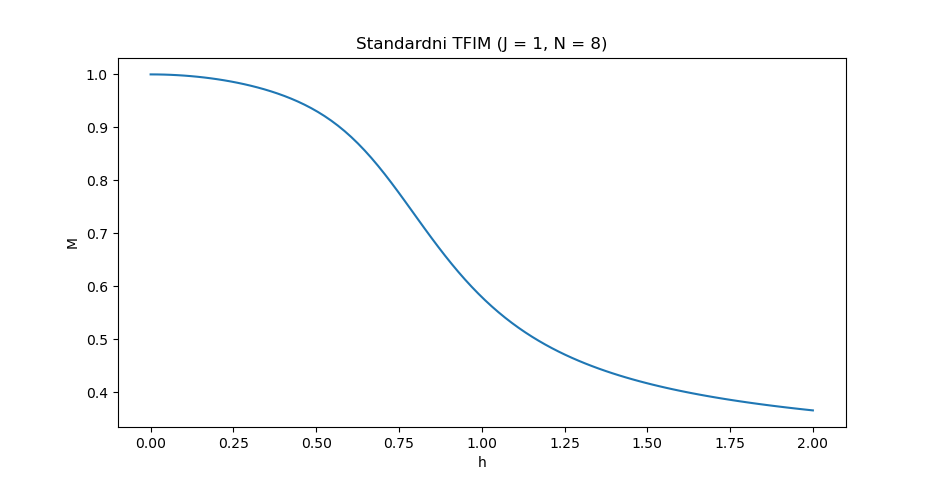
\includegraphics[width = \linewidth]{STFIM1.png}
    \caption{Graf magnetizacije v odvisnosti od h}
    \label{fig:enter-label}
\end{figure}




\noindent Če želimo videti, kako se, ko $N \rightarrow \infty$, magnetizacija približuje stopnici, si lahko obledamo tudi ta graf.
\begin{figure}[H]
    \centering
    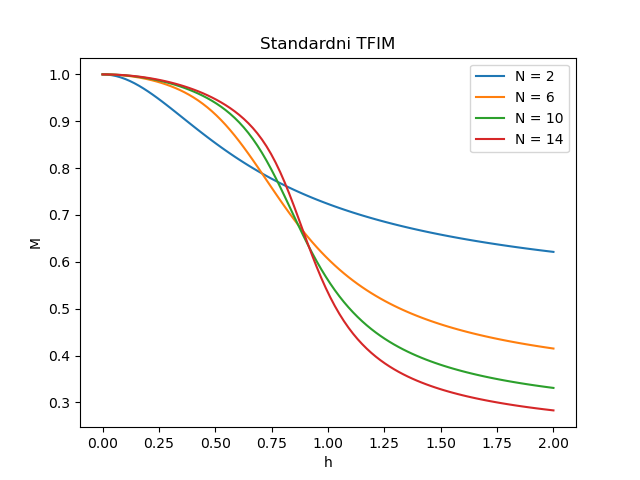
\includegraphics[width = \linewidth]{STFIM_variableN2.png}
    \caption{Graf magnetizacije v odvisnosti od h pri različnih N}
    \label{fig:enter-label}
\end{figure}

\newpage
\noindent Če variiramo oba J in h lahko narišemo naslednja 3D in contour grafa.
\begin{table}[H]
\begin{tabular}{c c}
     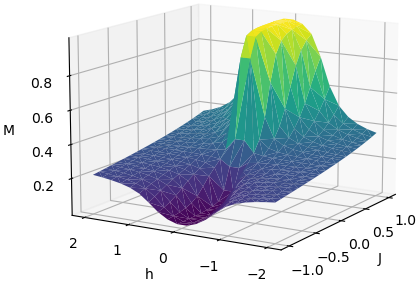
\includegraphics[width = .5 \linewidth]{STFIM2.png}
     &  
     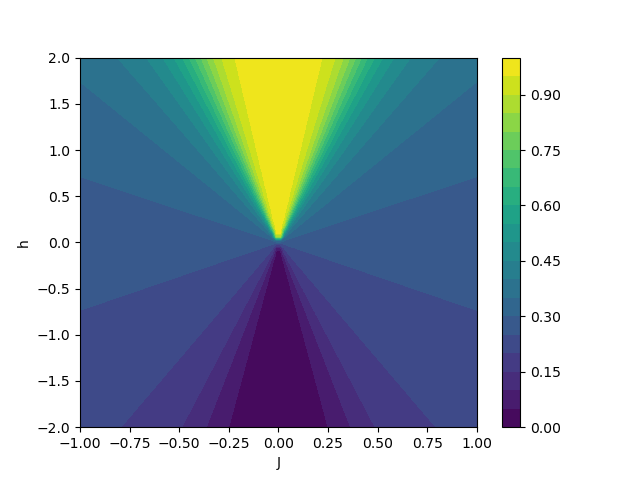
\includegraphics[width = .5 \linewidth]{STFIM3.png}\\
\end{tabular}
\caption*{Grafa magnetizacije v odvisnosti od h in J}
\end{table}

\noindent Na grafu lahko opazimo naslednje lastnosti:
\begin{itemize}
    \item Simetrija čez ravnino $h = 0$, kar ni nepričakovano, saj je veriga sama po sebi simetrična. Če polje obrnemo v drugo smer lahko zato pričakujemo, da bo rezultat le prezrcaljena rešitev za polje v prvotno smer. To pa ne vpliva na magnetizacijo, ki je "izpovprečena" čez celo verigo.  

    \item Če se osredotočimo na presek $h = 0$, vidimo, da se pri $J >> 0$ spini obnašajo kot feromagnet, saj so vsi spini poravnani. Za $J << 0$ pa lahko sumimo, da se obnaša kot antiferomagnet in so sosednji spini obrnjeni nasprotno. To lahko potrdimo, če izračunamo naslednjo količino in vidimo, da je zelo blizu 1.
    \begin{equation}
    |\frac{1}{N}\sum_{i=0}^N \sigma_i^z (-1)^i|
    \end{equation}
    \begin{figure}[H]
        \centering
         \includegraphics[]{STFIM_antiferomag.png}
        \caption{Graf mere za antiferomagnetizem v odvisnosti od J in h}
        \label{fig:enter-label}
    \end{figure}
   

    \item Na prvi pogled vidimo tudi, da se magnetizacija ustali a neki končni vrednosti okoli $0.2$, ko gre $h \rightarrow \infty$. To res velja za majhne sisteme, ampak za realne sisteme, kjer je $N \rightarrow \infty$, se ta končna vrednost bliža 0. To tendenco lahko vidimo v naslednjih grafih.

    \begin{table}[H]
    \hskip-1.2cm\begin{tabular}{c c}
        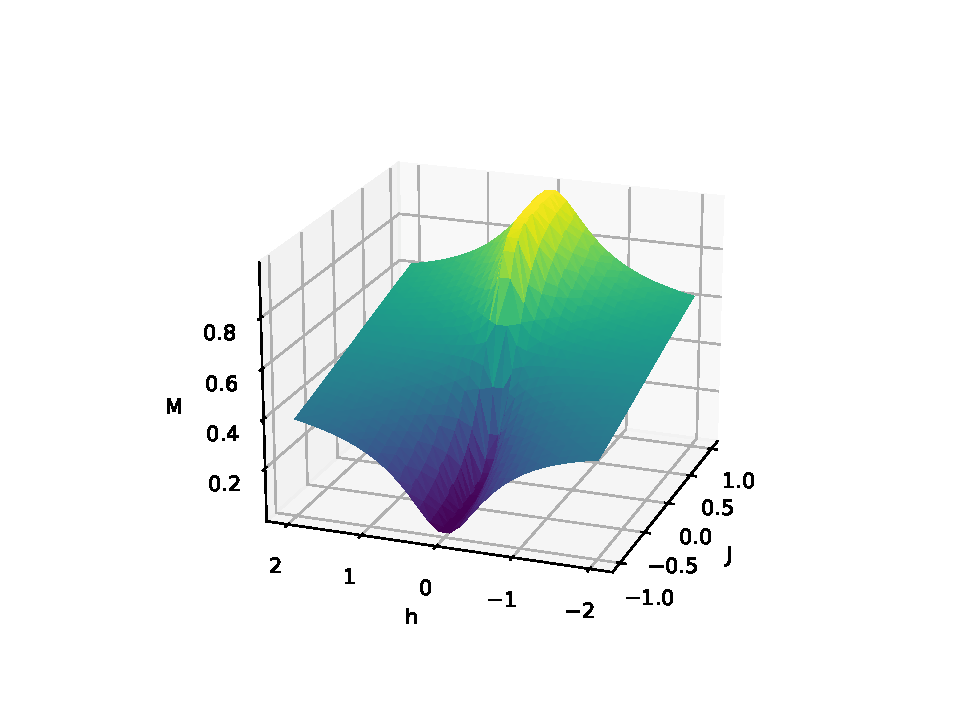
\includegraphics[trim=100 0 100 0,clip,width = .5 \textwidth]{TFIM_3D_N=2.pdf} &  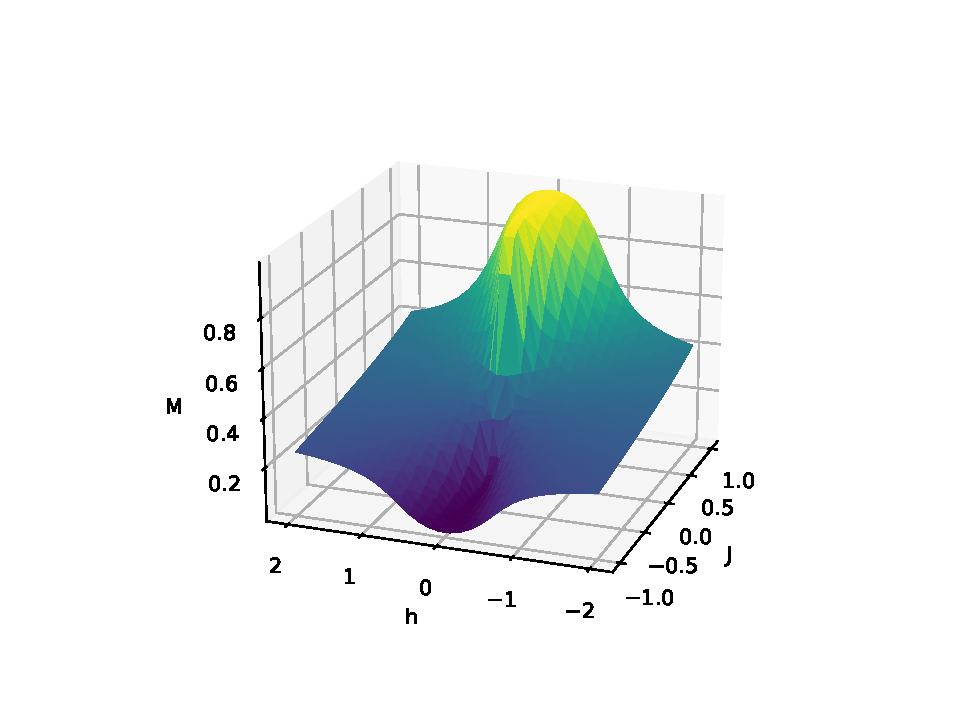
\includegraphics[trim=100 0 100 0,clip,width = .5 \textwidth]{TFIM_3D_N=6.pdf}\\
        N = 2& N = 6\\
        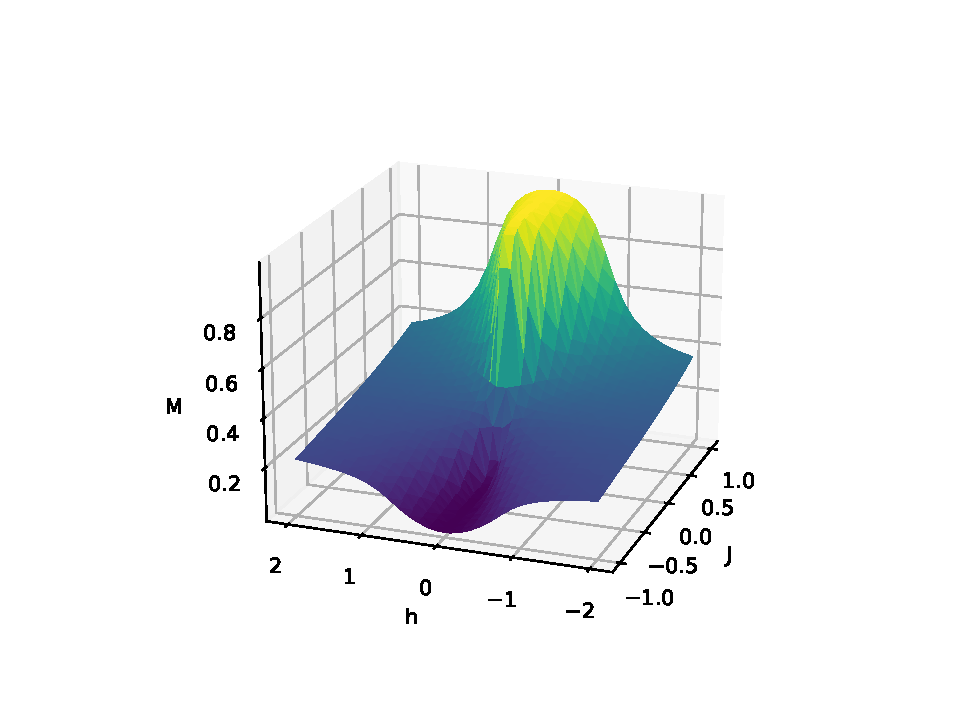
\includegraphics[trim=100 0 100 0,clip,width = .5 \textwidth]{TFIM_3D_N=8.pdf} &  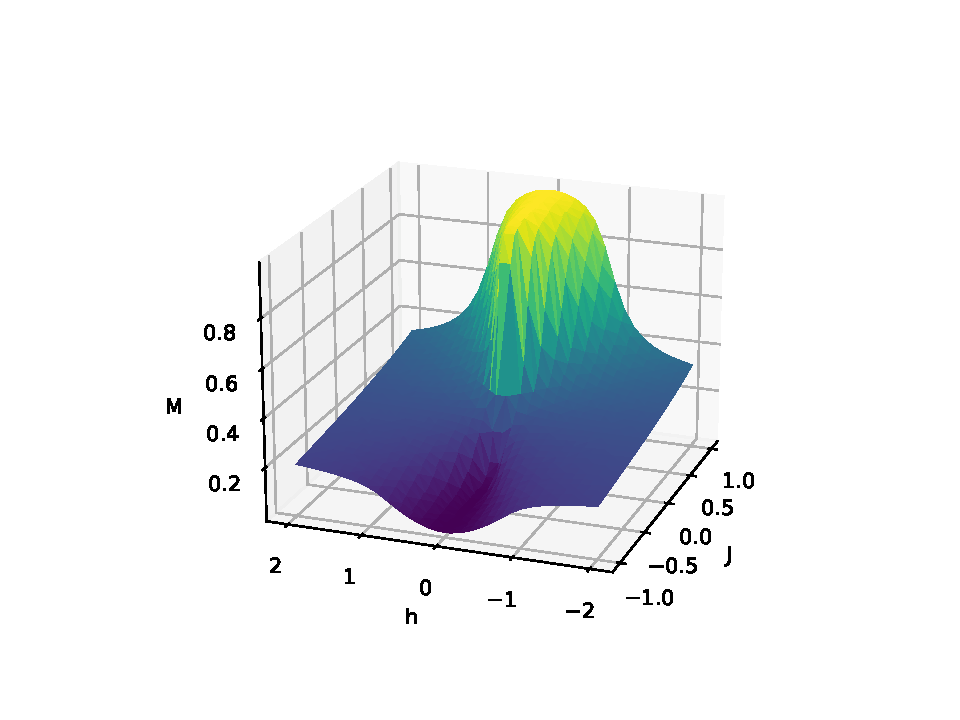
\includegraphics[trim=100 0 100 0,clip,width = .5 \textwidth]{TFIM_3D_N=10.pdf}\\
         N = 8 & N = 10 
    \end{tabular}
    \caption*{Grafi magnetizacije v odvisnosti od h in J pri različnih N}
    \end{table}
\end{itemize}



\section{Sklopljeni verigi}
\subsection{Eksaktna diagonalizacija}
Še malce bolj komplicirana varianta Isingovega modela je ta, ki nas tu v resnici zanima. Tega dobimo tako, da dve verigi spinov, za kateri velja TFIM, sklopimo med sabo. Hamiltonian tega modela se glasi:
\begin{equation}
    \hat{H} = \sum_{< i,j >} -J \hat{\sigma_{1i}^z} \hat{\sigma_{1j}^z} + \sum_{< i,j >} -J \hat{\sigma_{2i}^z} \hat{\sigma_{2j}^z} - h\sum_i \hat{\sigma_{1i}^x}- h\sum_i \hat{\sigma_{2i}^x} - J_T \sum_i \hat{\sigma_{1j}^z} \hat{\sigma_{2i}^z}
\end{equation}
Tudi pri tem problemu bomo spet uporabili isto bazo stanj. To pomeni, da vzamemo kot prej binarno reprezentacijo številke, le da tokrat prva polovica številke predstavlja eno verigo in druga polovica drugo. Ta baza je prikladna, ker lahko matriko hamiltoniana sestavimo na enak način kot prej.\\ 
Za dimenzije $N < 10$ lahko rešimo z direktno diagonalizacijo v doglednem času. Vse naslednje metode, predstavljene v tem poglavju se nahajajo v datoteki TFIM\_QuSpin\_2.py .
\subsection{Magnetizacija}
Dobra mera za stanje sistema, ki nas bo tu zanimala, je zoped magnetizacija, ki jo definiramo kot:
\begin{equation}
    M = \frac{1}{N}\sum_{i=0}^N \sigma_{1i}^z + \frac{1}{N}\sum_{i=0}^N \sigma_{2i}^z
\end{equation}\\

\noindent Če zoped variiramo $J$ in $h$, pri fiksnem $J_T = 1$ in $N = 8$, dobimo naslednji graf:

\begin{figure}[H]
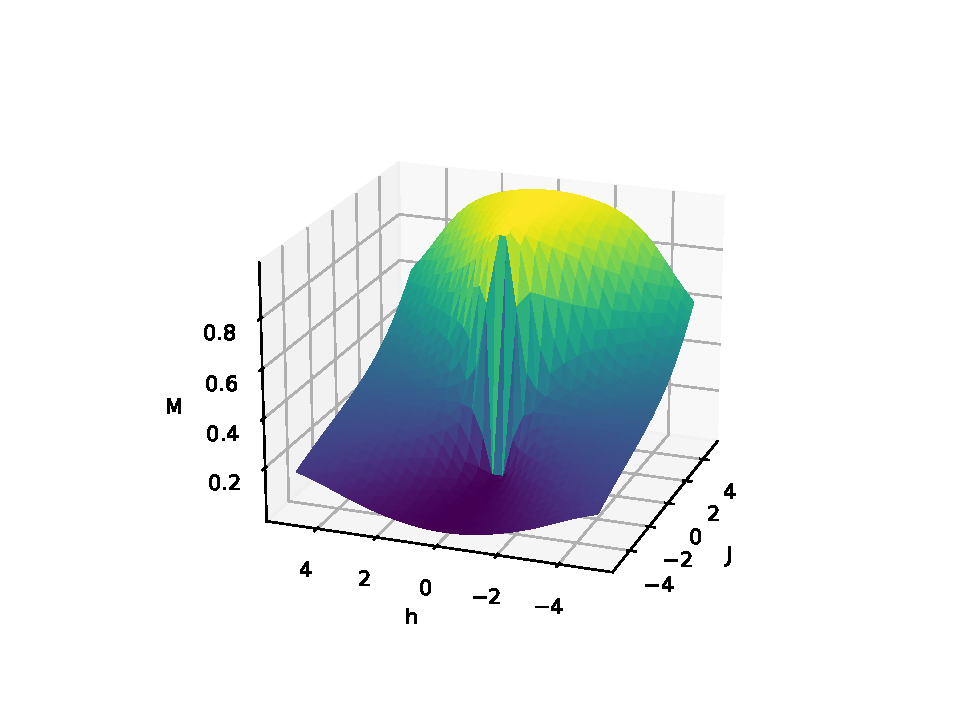
\includegraphics[]{TFIM2_3D_J_h_N=8.pdf}
\caption{Graf magnetizacije v odvisnosti od J in h, pri $J_T = 1$}
\end{figure}

\noindent Vidimo lahko, da se tudi ta model obnaša zelo podobno kot prvi. Glavna razlika, ki jo lahko opazimo je ta, da je sedaj prehod med feromagnetom in antiferomagnetom postal veliko ostrejši.\\\\

\noindent Če variiramo oba $h$ ter $J_T$ pri fiksnem $J = 1$, pa lahko narišemo naslednja 3D in contour grafa.

\begin{table}[H]
\begin{tabular}{cc}
     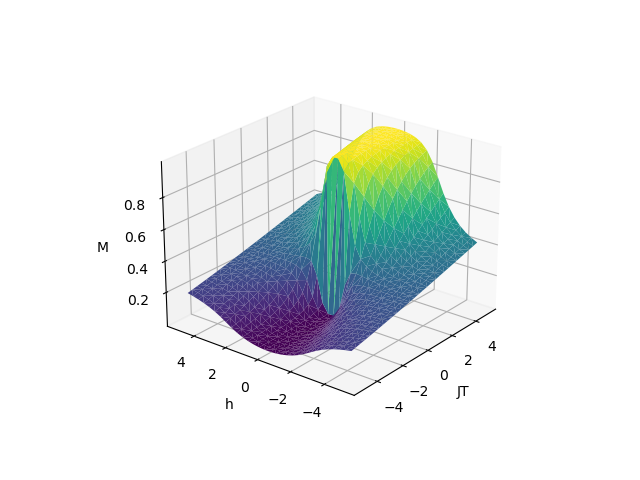
\includegraphics[trim = 100 20 100 0, clip ,width = .4 \linewidth]{2TFIM1.png}
     &  
     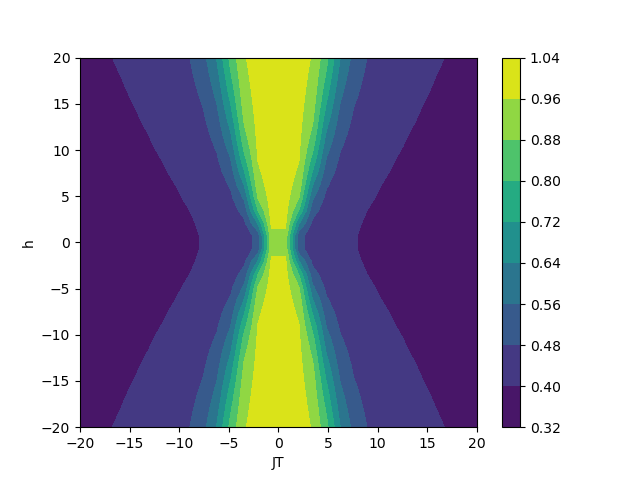
\includegraphics[width = .5 \linewidth]{2TFIM2.png}\\
\end{tabular}
\caption*{Grafa magnetizacije v odvisnosti od h in $J_T$, pri fiksnem $J = 1$}
\end{table}


\noindent Grafa ko je fiksen $J$ in ko je fiksen $J_T$ sta si zelo podobna. To je zato, ker si lahko, prav tako kot si sklopitev z $J_T$ predstavljamo kot dve verigi dolžine N naloženi ena na drugo, predstavljamo sklopitev z $J$ kot N verig dolžine 2, naloženih ena na drugo.

\section{Časovna evolucija sistema}
Še en način, poleg eksaktne diagonalizacije, s katerim se lahko dokopljemo do energije določenega lastnega stanja, je z uporabo adiabatičnega teorema, ki pravi, da če začnemo v lastnem stanju hamiltoniana in tega dovolj počasi spremijamo v drug hamiltonian, bomo na koncu v ustreznem lastnem stanju novega hamiltoniana. To pomeni, da lahko, če poznamo osnovno stanje enostavnega problema, kot je na primer navaden 1D Isingov model, lahko najdemo osnovno stanje kompleksnejšega TFIM modela, če zelo počasi prižigamo magnetno polje. Da bi tako dobili točno osnovno stanje, bi moralo biti to prižiganje neskončno počasno, vendar lahko tudi z končno počasnostjo dosežemo dober približek.

\subsection{Numerična integracija}

Za časovno evolucijo našega modela, moramo reševati Schrödingerjevo enačbo:
\begin{equation}
    \frac{\partial \vert v(t)\rangle}{\partial t} = -iH(t) \vert v(t) \rangle
\end{equation}
za kar bomo uporabili numerični integrator dop853, za katerim stoji Dormand-Prince metoda, eksplicitna Runge-Kutta metoda z adaptivno velikostjo koraka. Ta metoda ima zelo majhno napako glede na to kako hitra je, je pa res, da ni unitarna. To pomeni, da se zaradi numerične napake lahko pokvari normalizacija našega stanja, vendar je to v večini primerov zanemarljivo.\\\\
Naša naloga je sedaj izbrati primeren $H(t)$, ki poveže hamiltoniana naših dveh modelov in ki to stori na tak način, da v čim manjšem času dosežemo tem boljši približek osnovnega stanja kompleksnejšega modela To zvezo matematično zapišemo kot:
\begin{equation}
    H(t) = H_0 + f(t) \cdot \Delta H
\end{equation}
kjer sta $H_0$ in $\Delta H$ konstantni matriki in $f(t)$ funkcija, za katero velja, $f(t_0) = 0$ in $f(t_k) = 1$.\\\\
Na izbiro imamo seveda neštevno neskončno mnogo funkcij, jaz sem izbral tri, ki se zdijo naravne izbire:
\begin{equation}
    f(t) = kt \hspace{1cm} f(t) = e^{kt} \hspace{1cm} f(t) = \frac{1}{1+e^{-k_1(t-k2)}}
\end{equation}
Za zadnji dve izmed teh funkcij zahteve ne veljajo striktno, vendar se željenim vrednostim poljubno približajo. Za obe funkciji velja zahteva $f(t_0) = a$, za tretjo pa tudi $f(t_{max} = 1-a$\\\\

\subsection{Energija}
\noindent Numerična integracija nam vrne stanje sistema ob nekem končnem številu časov, ker nas zanima energija osnovnega stanja, moramo ta stanja pretvoriti v energije, to storimo preko formule:
\begin{equation}
E(t) = H(t)^T\vert v(t) \rangle H(t)    
\end{equation}

\begin{figure}[H]
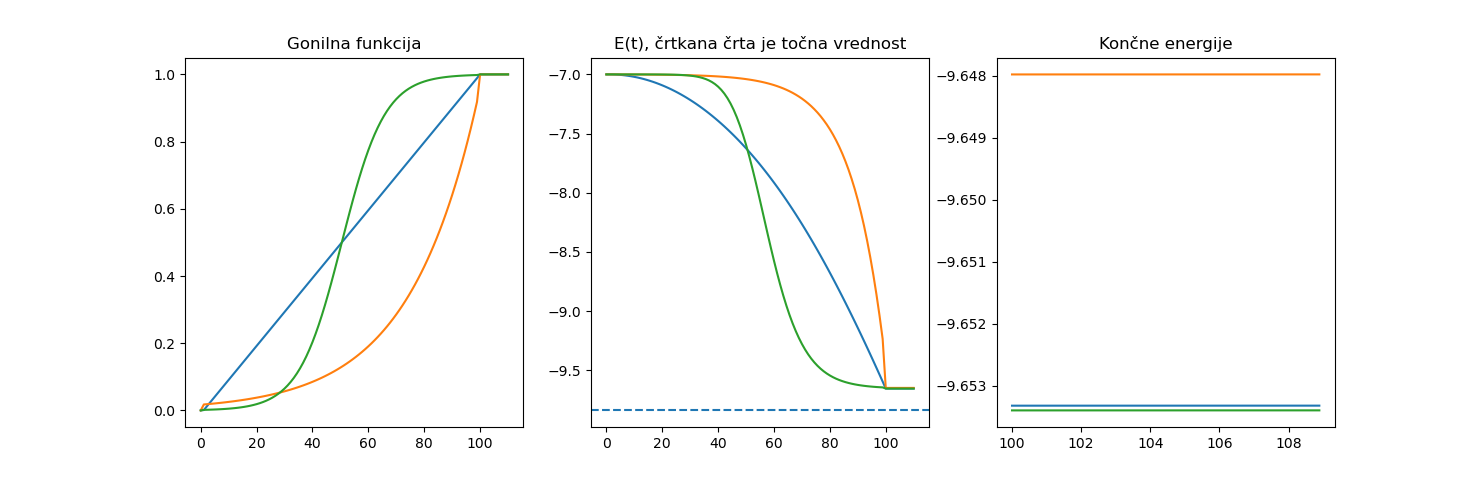
\includegraphics[width = \linewidth]{STFIM_Evolution.png}
\caption{Primerjava časovne evolucije z različnimi gonilnimi funkcijami}
\end{figure}

\begin{figure}[H]
    \centering
    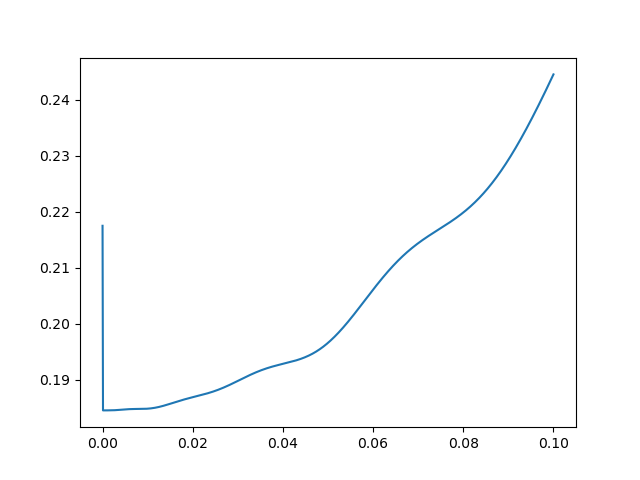
\includegraphics[width = \linewidth]{FermiDira.png}
    \caption{razlika med končno energijo in točno enerijo osnovnega stanja, za Fermi-Dirac gonilne funkcije z različnimi a}
    \label{fig:enter-label}
\end{figure}

\subsection{Skalarni produkt}
Še ena mera za prekrivanje valovnih funkcij je skalarni produkt. Na naslednjih grafih rišemo torej:
\begin{equation}
    \langle v(t) \vert \vert v_{eksaktno} \rangle
\end{equation}

\begin{figure}[H]
    \centering
    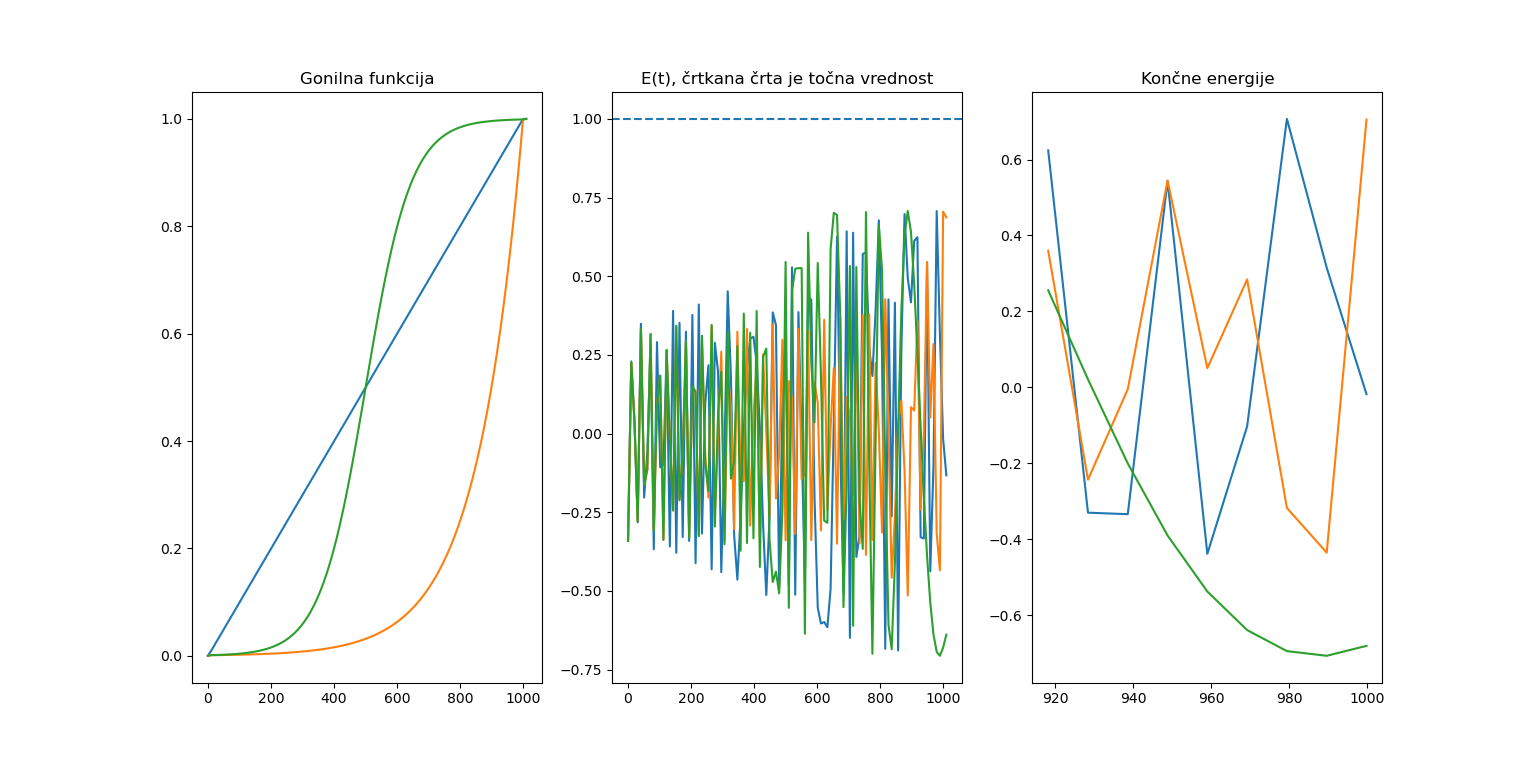
\includegraphics[width = \linewidth]{dot_various.png}
    \caption{Skalarni produkt}
    \label{fig:enter-label}
\end{figure}
\begin{figure}[H]
    \centering
    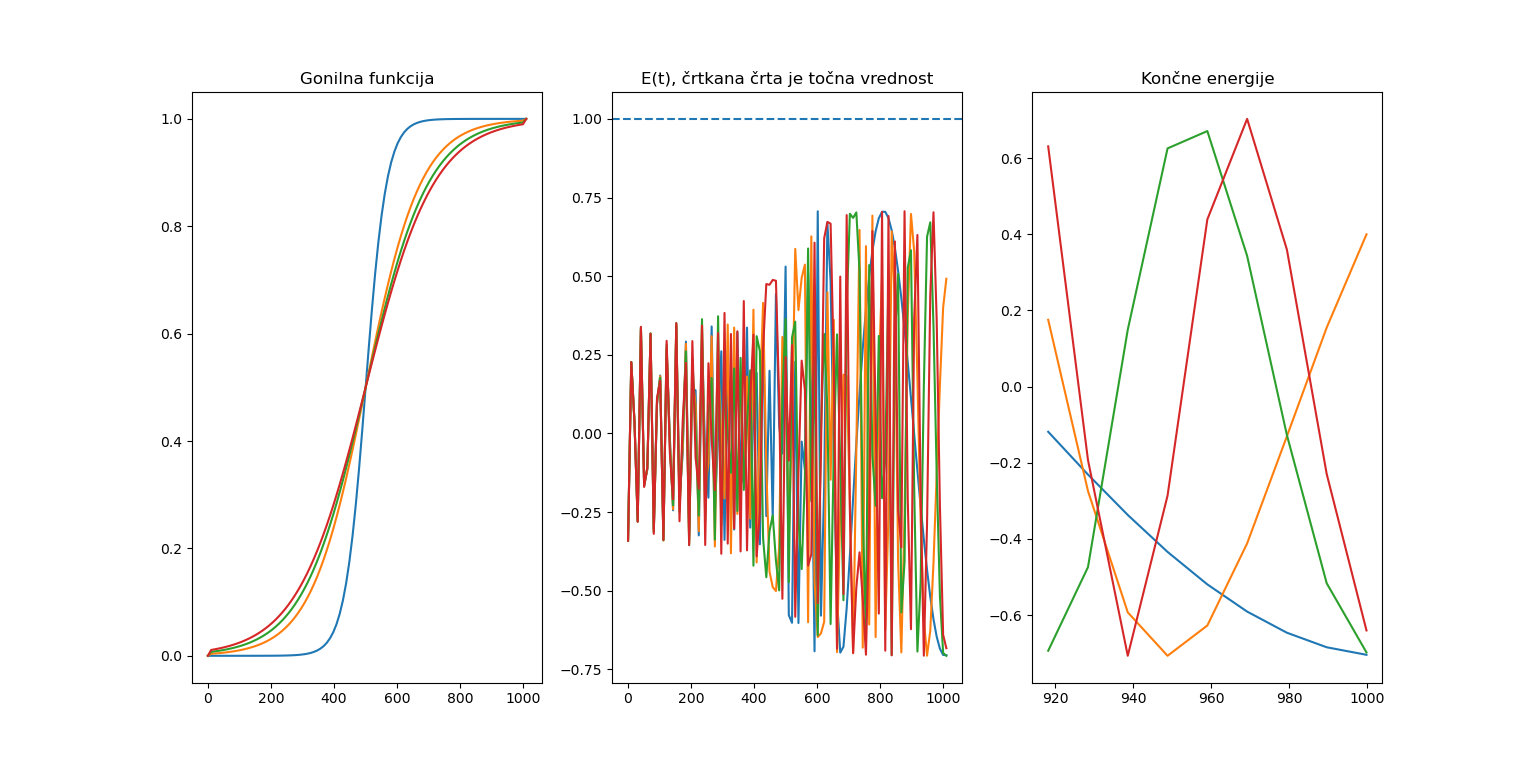
\includegraphics[width = \linewidth]{dot_fermis.png}
    \caption{Skalarni produkt}
    \label{fig:enter-label}
\end{figure}

\end{document}
